% preamble-exam-zh.tex — 共享 preamble
% 用于所有 exam-zh 模板
%
% 样式策略：
%   屏幕 → 语义彩色（蓝=关键想法，红=易错，绿=路线，灰=提示/教师备注）
%   打印 → 自动降级为黑白（通过 print mode 或 monochrome 选项）

\documentclass{exam-zh}

% ---------- 基础配置 ----------
\examsetup{
  page/size = a4paper,
  page/show-head = false,
  page/show-foot = false,
  sealline/show = false,
  font = times,
  math-font = xits,
}

\usepackage{tcolorbox}
\usepackage{needspace}
\tcbuselibrary{skins,breakable}

% ---------- 打印/屏幕颜色切换 ----------
% 用法：\documentclass[monochrome]{exam-zh} 即可切换为纯黑白
% 注意：不要使用 \if@xxx 放在 makeatother 外部；这里改成普通条件名。
\newif\ifeduprintcolor
\eduprintcolortrue

\makeatletter
\@ifclasswith{exam-zh}{monochrome}{\eduprintcolorfalse}{}
\makeatother

% ---------- 语义颜色定义 ----------
% 屏幕：有色彩区分；打印：降级为灰度
\ifeduprintcolor
  % --- 屏幕彩色模式 ---
  \definecolor{edu-blue}{RGB}{47, 82, 122}       % 关键想法
  \definecolor{edu-blue-bg}{RGB}{243, 246, 252}
  \definecolor{edu-red}{RGB}{180, 40, 40}         % 易错提醒
  \definecolor{edu-red-bg}{RGB}{255, 245, 240}
  \definecolor{edu-green}{RGB}{34, 100, 60}       % 路线图
  \definecolor{edu-green-bg}{RGB}{242, 250, 245}
  \definecolor{edu-orange}{RGB}{160, 90, 0}       % 训练目标
  \definecolor{edu-orange-bg}{RGB}{255, 248, 235}
  \definecolor{edu-gray}{RGB}{100, 100, 100}      % 提示/教师备注
  \definecolor{edu-gray-bg}{RGB}{248, 248, 248}
  \definecolor{edu-purple}{RGB}{90, 50, 120}      % 思考题
  \definecolor{edu-purple-bg}{RGB}{248, 244, 252}
\else
  % --- 打印黑白模式 ---
  \definecolor{edu-blue}{gray}{0.15}
  \definecolor{edu-blue-bg}{gray}{0.96}
  \definecolor{edu-red}{gray}{0.25}
  \definecolor{edu-red-bg}{gray}{0.97}
  \definecolor{edu-green}{gray}{0.20}
  \definecolor{edu-green-bg}{gray}{0.97}
  \definecolor{edu-orange}{gray}{0.25}
  \definecolor{edu-orange-bg}{gray}{0.98}
  \definecolor{edu-gray}{gray}{0.40}
  \definecolor{edu-gray-bg}{gray}{0.97}
  \definecolor{edu-purple}{gray}{0.30}
  \definecolor{edu-purple-bg}{gray}{0.98}
\fi

% ---------- 自定义教学环境 ----------
% 共性：enhanced + breakable（跨页不断裂）

% 原题卡片 — 强边框，突出显示
\newtcolorbox{problemcard}{
  enhanced, breakable,
  colback=edu-blue-bg,
  colframe=edu-blue,
  boxrule=1.2pt,
  arc=0pt,
  left=3mm, right=3mm, top=3mm, bottom=3mm,
}

% 解题路线图 — 左边线 + 浅底
\newtcolorbox{routebox}{
  enhanced, breakable,
  colback=edu-green-bg,
  colframe=edu-green!30,
  boxrule=0pt,
  borderline west={2.5pt}{0pt}{edu-green},
  left=3mm, right=3mm, top=3mm, bottom=3mm,
}

% 关键想法 — 蓝色左边线
\newtcolorbox{keyideabox}{
  enhanced, breakable,
  colback=edu-blue-bg,
  colframe=edu-blue!30,
  boxrule=0pt,
  borderline west={2.5pt}{0pt}{edu-blue},
  left=3mm, right=3mm, top=3mm, bottom=3mm,
}

% 易错提醒 — 红色左边线
\newtcolorbox{mistakebox}{
  enhanced, breakable,
  colback=edu-red-bg,
  colframe=edu-red!20,
  boxrule=0pt,
  borderline west={3pt}{0pt}{edu-red},
  left=3mm, right=3mm, top=2.5mm, bottom=2.5mm,
}

% 提示 — 灰色虚线左边线
\newtcolorbox{hintbox}{
  enhanced, breakable,
  colback=edu-gray-bg,
  colframe=edu-gray!20,
  boxrule=0pt,
  borderline west={2pt}{0pt}{edu-gray, dashed},
  left=3mm, right=3mm, top=2mm, bottom=2mm,
}

% 思考题 — 紫色虚线左边线
\newtcolorbox{thinkbox}{
  enhanced, breakable,
  colback=edu-purple-bg,
  colframe=edu-purple!20,
  boxrule=0pt,
  borderline west={2pt}{0pt}{edu-purple, dashed},
  left=2.5mm, right=2.5mm, top=2.5mm, bottom=2.5mm,
}

% 教师备注 — 灰色左边线，小字
\newtcolorbox{teachernote}{
  enhanced, breakable,
  colback=edu-gray-bg,
  colframe=edu-gray!15,
  boxrule=0pt,
  borderline west={2pt}{0pt}{edu-gray!60},
  left=2.5mm, right=2.5mm, top=2.5mm, bottom=2.5mm,
  fontupper=\small,
  colupper=black!60,
}

% 训练目标 — 橙色左边线，小字
\newtcolorbox{traininggoal}{
  enhanced, breakable,
  colback=edu-orange-bg,
  colframe=edu-orange!15,
  boxrule=0pt,
  borderline west={1.5pt}{0pt}{edu-orange},
  left=2mm, right=2mm, top=1mm, bottom=1mm,
  fontupper=\small,
}

% 答题区 — 无边框，纯留白
\newcommand{\answerarea}[1][40mm]{%
  \vspace{2mm}%
  \begin{tcolorbox}[
    enhanced, breakable,
    colback=white,
    colframe=white,
    boxrule=0pt,
    height=#1,
    valign=top,
    bottom=0mm,
    after skip=0mm,
  ]
  \end{tcolorbox}%
}

% ---------- 字体设置 ----------
% exam-zh (ctexbook) already sets CJK fonts via ctex.
% Only override if specific fonts are needed.
% macOS: Songti SC, STHeiti, STFangsong
% Linux: SimSun, SimHei, FangSong

% ---------- 页面设置 ----------
% exam-zh (ctexbook) already loads geometry.
% Override margins if needed:
% \geometry{top=16mm, bottom=16mm, left=14mm, right=14mm}

\examsetup{
  question/show-answer = true,
  fillin/show-answer = true,
  solution/show-solution = show-stay,
}

% ---------- 教师版解答样式 ----------
\newtcolorbox{solutionblock}{
  enhanced, breakable,
  colback=edu-blue-bg,
  colframe=edu-blue!25,
  boxrule=0pt,
  borderline west={2pt}{0pt}{edu-blue!50},
  arc=0pt,
  left=3mm, right=3mm, top=2mm, bottom=2mm,
  before skip=2mm,
  after skip=3mm,
  fontupper=\small,
}

% 解答步骤编号
\newcounter{solstep}
\newcommand{\solstep}[2]{%
  \stepcounter{solstep}%
  \par\medskip
  \noindent\hangindent=6mm
  {\color{edu-blue}\bfseries\textcircled{\scriptsize\thesolstep}\enspace #1}\enspace #2\par
}

\begin{document}

\section*{一次函数图像与一元一次不等式 · 专题练习（教师版）}

\section*{一、选择题（每题 4 分，共 12 分）}


\begin{question}[points=4]
  已知一次函数 $y = k_1x + b_1$ 的图像与 $y = k_2x + b_2$ 的图像交于点 $P(-2, 3)$，且 $y = k_1x + b_1$ 随 $x$ 的增大而增大，$y = k_2x + b_2$ 随 $x$ 的增大而减小。则不等式 $k_1x + b_1 < k_2x + b_2$ 的解集是
  \begin{choices}
    \item $x > -2$
    \item $x < -2$
    \item $x > 3$
    \item $x < 3$
  \end{choices}
  \paren[B]
  \begin{solutionblock}
    因为直线 $y = k_1x + b_1$ 随 $x$ 的增大而增大，所以该直线为递增直线（向右上倾斜）；
因为直线 $y = k_2x + b_2$ 随 $x$ 的增大而减小，所以该直线为递减直线（向右下倾斜）。
两条直线相交于点 $P(-2, 3)$，所以在交点的左侧（即 $x < -2$ 时），递增直线在递减直线的下方，
即 $k_1x + b_1 < k_2x + b_2$。因此解集为 $x < -2$。

  \end{solutionblock}
\end{question}



\begin{question}[points=4]
  已知一次函数 $y = 2x + k$ 的图像与直线 $y = -x + 3$ 交于点 $P(a, 2)$，则关于 $x$ 的不等式 $2x + k \ge -x + 3$ 的解集为
  \begin{choices}
    \item $x \ge 1$
    \item $x \le 1$
    \item $x \ge 2$
    \item $x \le 2$
  \end{choices}
  \paren[A]
  \begin{solutionblock}
    因为交点 $P(a, 2)$ 在已知直线 $y = -x + 3$ 上，代入得 $2 = -a + 3$，解得 $a = 1$。
故两直线交点为 $P(1, 2)$，交点横坐标为 $x = 1$。
不等式 $2x + k \ge -x + 3$ 意味着直线 $y = 2x + k$ 在直线 $y = -x + 3$ 的上方。
因为 $2 > 0$（递增），$-1 < 0$（递减），所以当 $x \ge 1$ 时，递增的直线在递减直线的上方或重合。
故解集为 $x \ge 1$。

  \end{solutionblock}
\end{question}



\begin{question}[points=4]
  若一次函数 $y = kx + b$ 的图像经过第一、二、四象限，且与直线 $y = x + 1$ 相交于点 $P(1, 2)$，则关于 $x$ 的不等式 $x + 1 > kx + b$ 的解集是
  \begin{choices}
    \item $x > 1$
    \item $x < 1$
    \item $x > 2$
    \item $x < 2$
  \end{choices}
  \paren[A]
  \begin{solutionblock}
    因为直线 $y = kx + b$ 经过第一、二、四象限，所以该直线的斜率 $k < 0$，直线向右下方倾斜。
而直线 $y = x + 1$ 的斜率为 $1 > 0$，向右上方倾斜。
两条直线相交于点 $P(1, 2)$，在交点右侧（即 $x > 1$ 时），向右上方倾斜的直线 $y = x + 1$ 在向右下方倾斜的直线 $y = kx + b$ 的上方，
即 $x + 1 > kx + b$。因此不等式的解集为 $x > 1$。

  \end{solutionblock}
\end{question}


\section*{二、填空题（每题 4 分，共 12 分）}


\begin{question}[points=4]
  已知一次函数 $y = 3x - 2$ 与 $y = x + 4$ 的图像交点坐标为 \underline{\quad\quad}。
  \paren[$(3, 7)$]
  \begin{solutionblock}
    联立两解析式得：$3x - 2 = x + 4$。
解得 $2x = 6 \implies x = 3$。
将 $x = 3$ 代入 $y = x + 4$ 得 $y = 7$。
所以交点坐标为 $(3, 7)$。

  \end{solutionblock}
\end{question}



\begin{question}[points=4]
  已知一次函数 $y = kx + b$ 与正比例函数 $y = -2x$ 的图像相交于点 $P(-1, m)$，且一次函数 $y = kx + b$ 的图像与 $y$ 轴交点为 $(0, 4)$，则该一次函数的解析式为 \underline{\quad\quad}。
  \paren[$y = 2x + 4$]
  \begin{solutionblock}
    将点 $P(-1, m)$ 代入正比例函数 $y = -2x$，得 $m = -2 \times (-1) = 2$。
故交点坐标为 $P(-1, 2)$。
因为一次函数 $y = kx + b$ 与 $y$ 轴的交点为 $(0, 4)$，所以 $b = 4$。
再将点 $P(-1, 2)$ 代入 $y = kx + 4$ 得：$2 = -k + 4$，解得 $k = 2$。
所以该解析式为 $y = 2x + 4$。

  \end{solutionblock}
\end{question}



\begin{question}[points=4]
  已知直线 $l_1: y = 2x + 6$ 与直线 $l_2: y = kx + b$ 相交于点 $P(-2, 2)$，且直线 $l_2$ 与 $y$ 轴交于点 $(0, -2)$，则不等式 $2x + 6 \le kx + b$ 的解集是 \underline{\quad\quad}。
  \paren[$x \le -2$]
  \begin{solutionblock}
    直线 $l_2$ 经过 $P(-2, 2)$ 和 $(0, -2)$，可求得其斜率 $k = \frac{-2 - 2}{0 - (-2)} = -2 < 0$，直线向右下倾斜。
直线 $l_1$ 的斜率为 $2 > 0$，向右上倾斜。
它们相交于 $P(-2, 2)$，在交点左侧（即 $x \le -2$ 时），向右上倾斜的直线 $l_1$ 位于向右下倾斜的直线 $l_2$ 的下方或与之重合。
即 $2x + 6 \le kx + b$。因此解集为 $x \le -2$。

  \end{solutionblock}
\end{question}


\section*{三、解答题（每题 12 分，共 36 分）}

\needspace{8\baselineskip}

\begin{problem}[points=12]
  如图 1，已知一次函数 $y = -x + 3$ 的图像 $l_1$ 与另一个一次函数 $y = kx + b$ 的图像 $l_2$ 相交于点 $P(1, 2)$，且 $l_2$ 经过点 $A(0, -1)$。
\begin{center}
  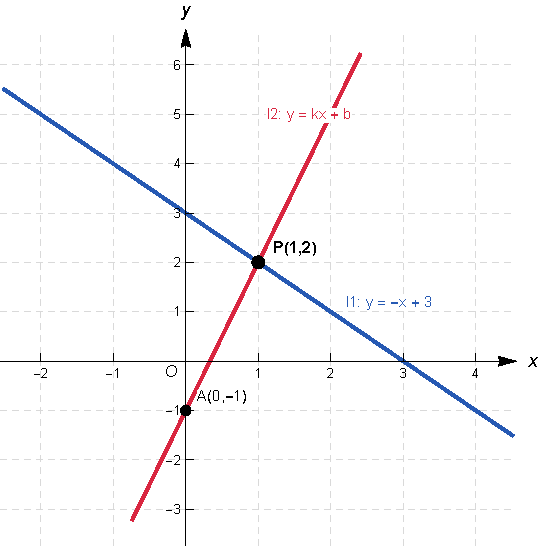
\includegraphics[width=6.5cm]{plot_p1.pdf}
\end{center}
\begin{enumerate}[label=(\arabic*)]
  \item 求一次函数 $y = kx + b$ 的解析式；
  \item 直接根据图像，求不等式 $kx + b > -x + 3$ 的解集；
  \item 求直线 $l_2$ 与坐标轴围成的三角形面积。
\end{enumerate}

  \setcounter{solstep}{0}
  \begin{solutionblock}
    \textbf{答案：}(1) $y = 3x - 1$；(2) $x > 1$；(3) $\frac{1}{6}$。\par\medskip
    \solstep{待定系数法求解析式}{}
    \solstep{}{因为直线过 $A(0, -1)$，故 $b = -1$。代入 $P(1, 2)$ 得 $2 = k - 1 \implies k = 3$。所以解析式为 $y = 3x - 1$。}
    \solstep{数形结合读解集}{}
    \solstep{}{观察图像发现，在交点 $P(1, 2)$ 右侧直线 $l_2$ 在直线 $l_1$ 的上方，因此不等式 $kx + b > -x + 3$ 的解集为 $x > 1$。}
    \solstep{计算坐标轴交点与面积}{}
    \solstep{}{令 $y = 0$ 得 $x = \frac{1}{3}$，与 $x$ 轴交于 $(\frac{1}{3}, 0)$，与 $y$ 轴交于 $(0, -1)$。面积为 $S = \frac{1}{2} \times 1 \times \frac{1}{3} = \frac{1}{6}$。}
  \end{solutionblock}
\end{problem}


\needspace{8\baselineskip}

\begin{problem}[points=12]
  如图 2，已知一次函数 $y = x - 1$ 的图像 $l_1$ 与另一个一次函数 $y = kx + b$ 的图像 $l_2$ 相交于点 $P(2, 1)$，且 $l_2$ 经过点 $B(0, 5)$。
\begin{center}
  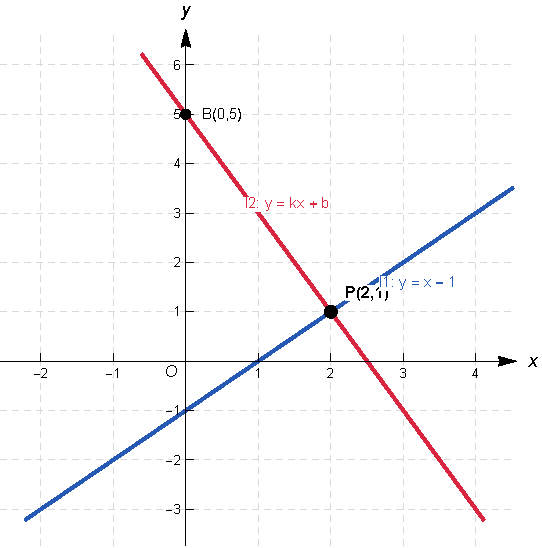
\includegraphics[width=6.5cm]{plot_p2.pdf}
\end{center}
\begin{enumerate}[label=(\arabic*)]
  \item 求一次函数 $y = kx + b$ 的解析式；
  \item 直接根据图像，求不等式 $kx + b \ge x - 1$ 的解集；
  \item 求直线 $l_1, l_2$ 与 $y$ 轴围成的三角形面积。
\end{enumerate}

  \setcounter{solstep}{0}
  \begin{solutionblock}
    \textbf{答案：}(1) $y = -2x + 5$；(2) $x \le 2$；(3) 6。\par\medskip
    \solstep{求一次函数解析式}{}
    \solstep{}{直线 $l_2$ 过点 $B(0, 5) \implies b = 5$。代入 $P(2, 1)$ 得 $1 = 2k + 5 \implies k = -2$。故解析式为 $y = -2x + 5$。}
    \solstep{求不等式解集}{}
    \solstep{}{观察图形知，$l_2$ 位于 $l_1$ 上方对应的区间（包括相交点）在 $x = 2$ 左侧，故解集为 $x \le 2$。}
    \solstep{计算两线与 y 轴所围面积}{}
    \solstep{}{两线与 $y$ 轴交点分别为 $(0, -1)$ 和 $(0, 5)$，底为 $6$；交点 $P(2, 1)$ 横坐标为 $2$，高为 $2$。面积 $S = \frac{1}{2} \times 6 \times 2 = 6$。}
  \end{solutionblock}
\end{problem}


\needspace{8\baselineskip}

\begin{problem}[points=12]
  如图 3，已知一次函数 $y = 2x + 4$ 的图像 $l_1$ 与另一个一次函数 $y = kx + b$ 的图像 $l_2$ 相交于点 $P(-1, 2)$，且 $l_2$ 经过点 $C(0, 3)$。
\begin{center}
  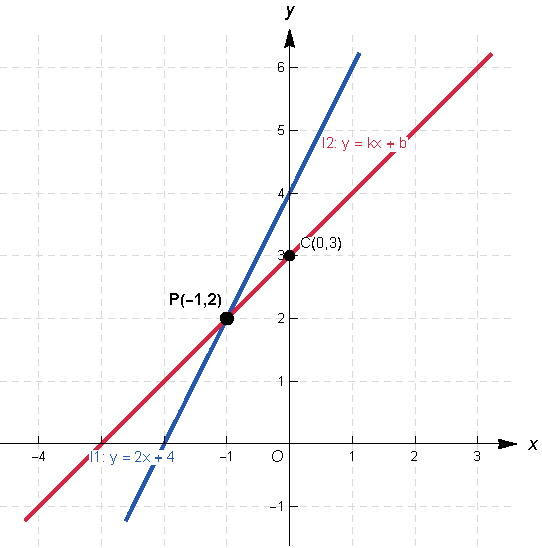
\includegraphics[width=6.5cm]{plot_p3.pdf}
\end{center}
\begin{enumerate}[label=(\arabic*)]
  \item 求一次函数 $y = kx + b$ 的解析式；
  \item 直接根据图像，求不等式 $2x + 4 < kx + b$ 的解集；
  \item 直线 $l_1, l_2$ 分别与 $x$ 轴相交于点 $A$ 和点 $B$，求 $\triangle PAB$ 的面积。
\end{enumerate}

  \setcounter{solstep}{0}
  \begin{solutionblock}
    \textbf{答案：}(1) $y = x + 3$；(2) $x < -1$；(3) 1。\par\medskip
    \solstep{求待定系数及解析式}{}
    \solstep{}{$l_2$ 过 $C(0, 3) \implies b = 3$。代入 $P(-1, 2)$ 得 $2 = -k + 3 \implies k = 1$。故解析式为 $y = x + 3$。}
    \solstep{求不等式解集}{}
    \solstep{}{从图像可以看出，在交点 $P(-1, 2)$ 左侧，直线 $l_2$ 在直线 $l_1$ 的上方，所以 $2x + 4 < kx + b$ 的解集为 $x < -1$。}
    \solstep{求与 x 轴交点及三角形面积}{}
    \solstep{}{令 $y = 0$：$l_1$ 交 $x$ 轴于 $A(-2, 0)$，$l_2$ 交 $x$ 轴于 $B(-3, 0)$。底边 $AB = 1$。高为 $P$ 的纵坐标 $2$。面积 $S = \frac{1}{2} \times 1 \times 2 = 1$。}
  \end{solutionblock}
\end{problem}


\clearpage
\section*{参考答案}


\begin{keyideabox}
  \textbf{选择题}
  1. B（$x < -2$）
2. A（$x \ge 1$）
3. A（$x > 1$）

\end{keyideabox}



\begin{keyideabox}
  \textbf{填空题}
  1. $(3, 7)$
2. $y = 2x + 4$
3. $x \le -2$

\end{keyideabox}



\begin{keyideabox}
  \textbf{解答题}
  第 1 题：(1) $y = 3x - 1$；(2) $x > 1$；(3) $\frac{1}{6}$。
第 2 题：(1) $y = -2x + 5$；(2) $x \le 2$；(3) 6。
第 3 题：(1) $y = x + 3$；(2) $x < -1$；(3) 1。

\end{keyideabox}



\end{document}
